\section{Characterisation of the Temperature Homogeneity}
\label{appendix:chuck_temp}

\begin{equation}
    \label{eq:temp_scaling}
    \frac{I}{T^2}\cdot \exp{\frac{E_g}{2\cdot k_b \cdot T}}~\equiv~\text{const.}
\end{equation}

\begin{figure}[h]
	\centering
	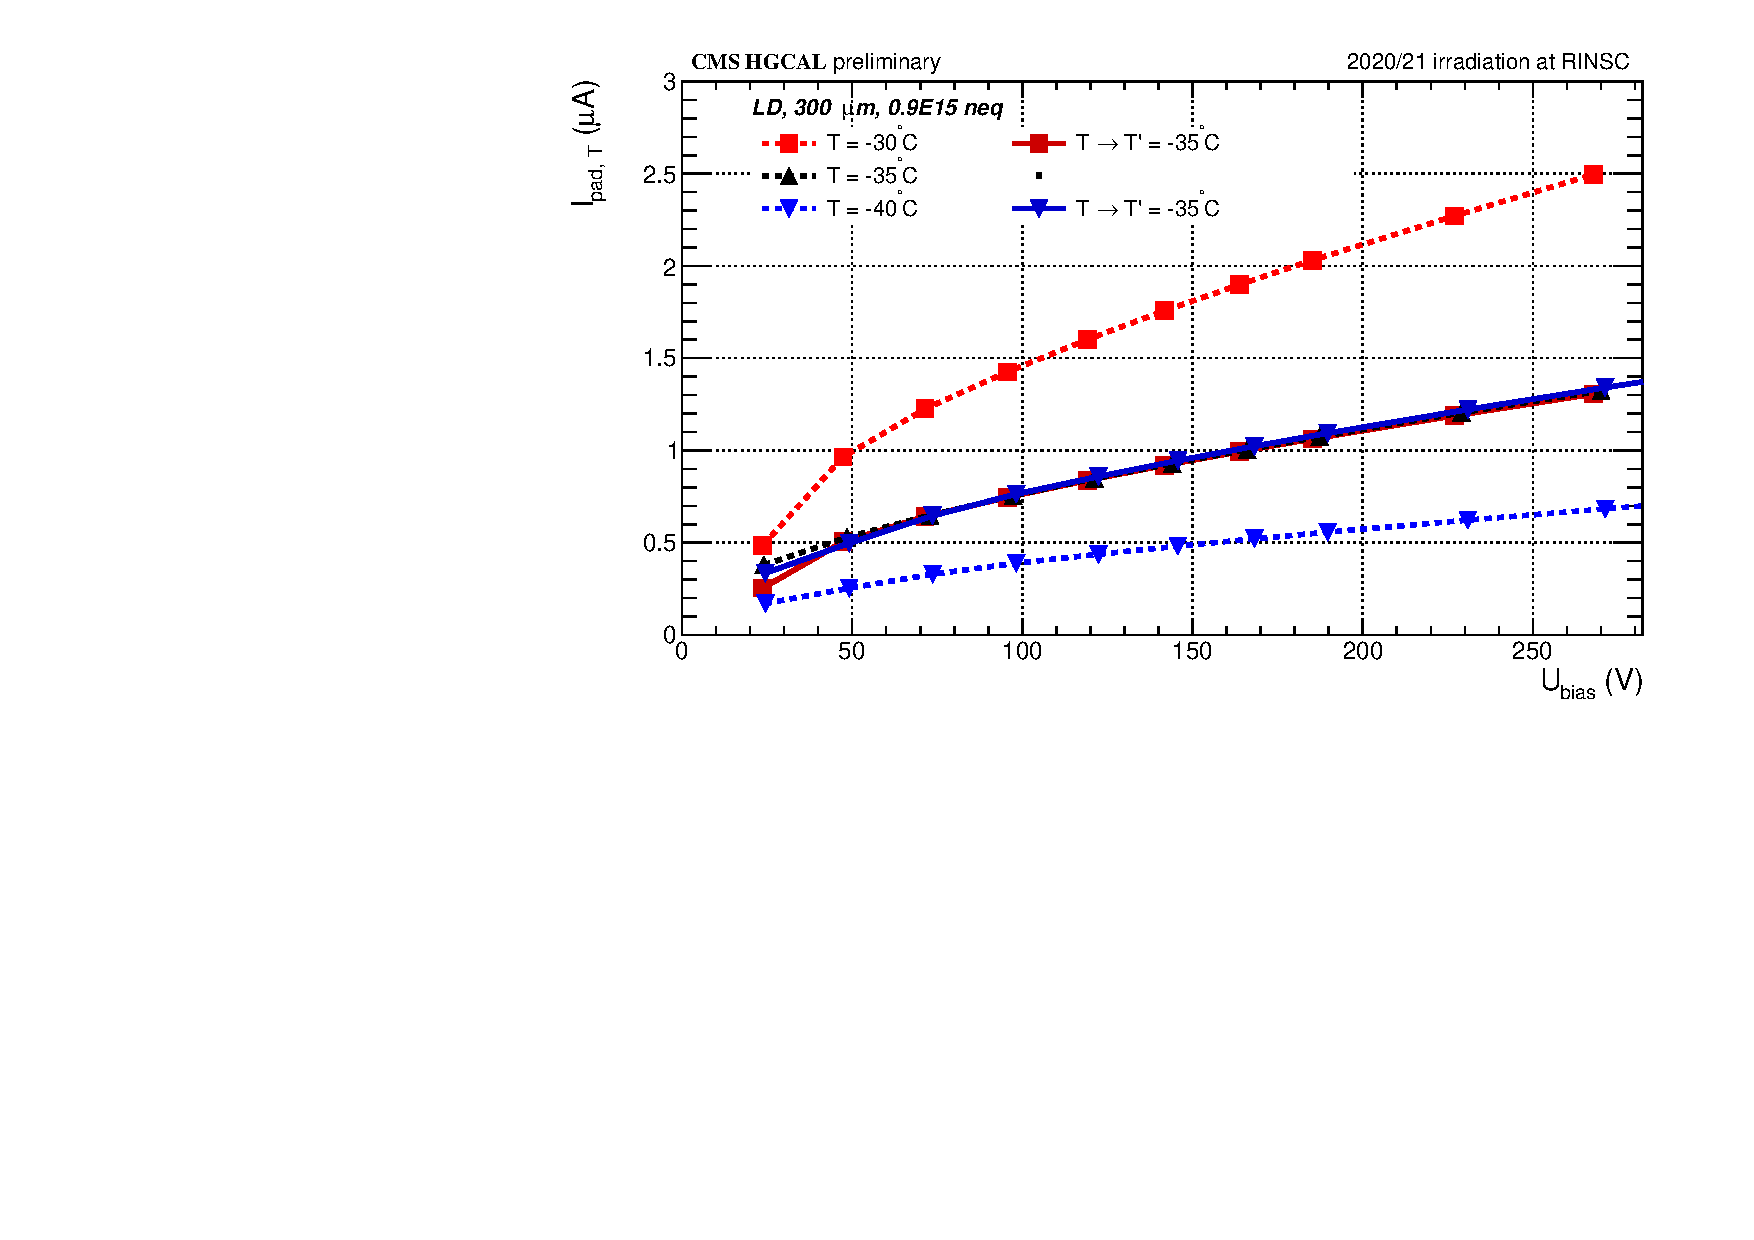
\includegraphics[width=0.49\textwidth]{plots/iv_temp_scaling/iv_overlay_ch24.pdf}
	\label{plot:iv_tempscaling}
	\caption{
	    Validation of temperature scaling formula, cf. ~\ref{eq:temp_scaling}.
	}
\end{figure}

\begin{figure}
	\captionsetup[subfigure]{aboveskip=-1pt,belowskip=-1pt}
	\centering
	\begin{subfigure}[b]{0.32\textwidth}
		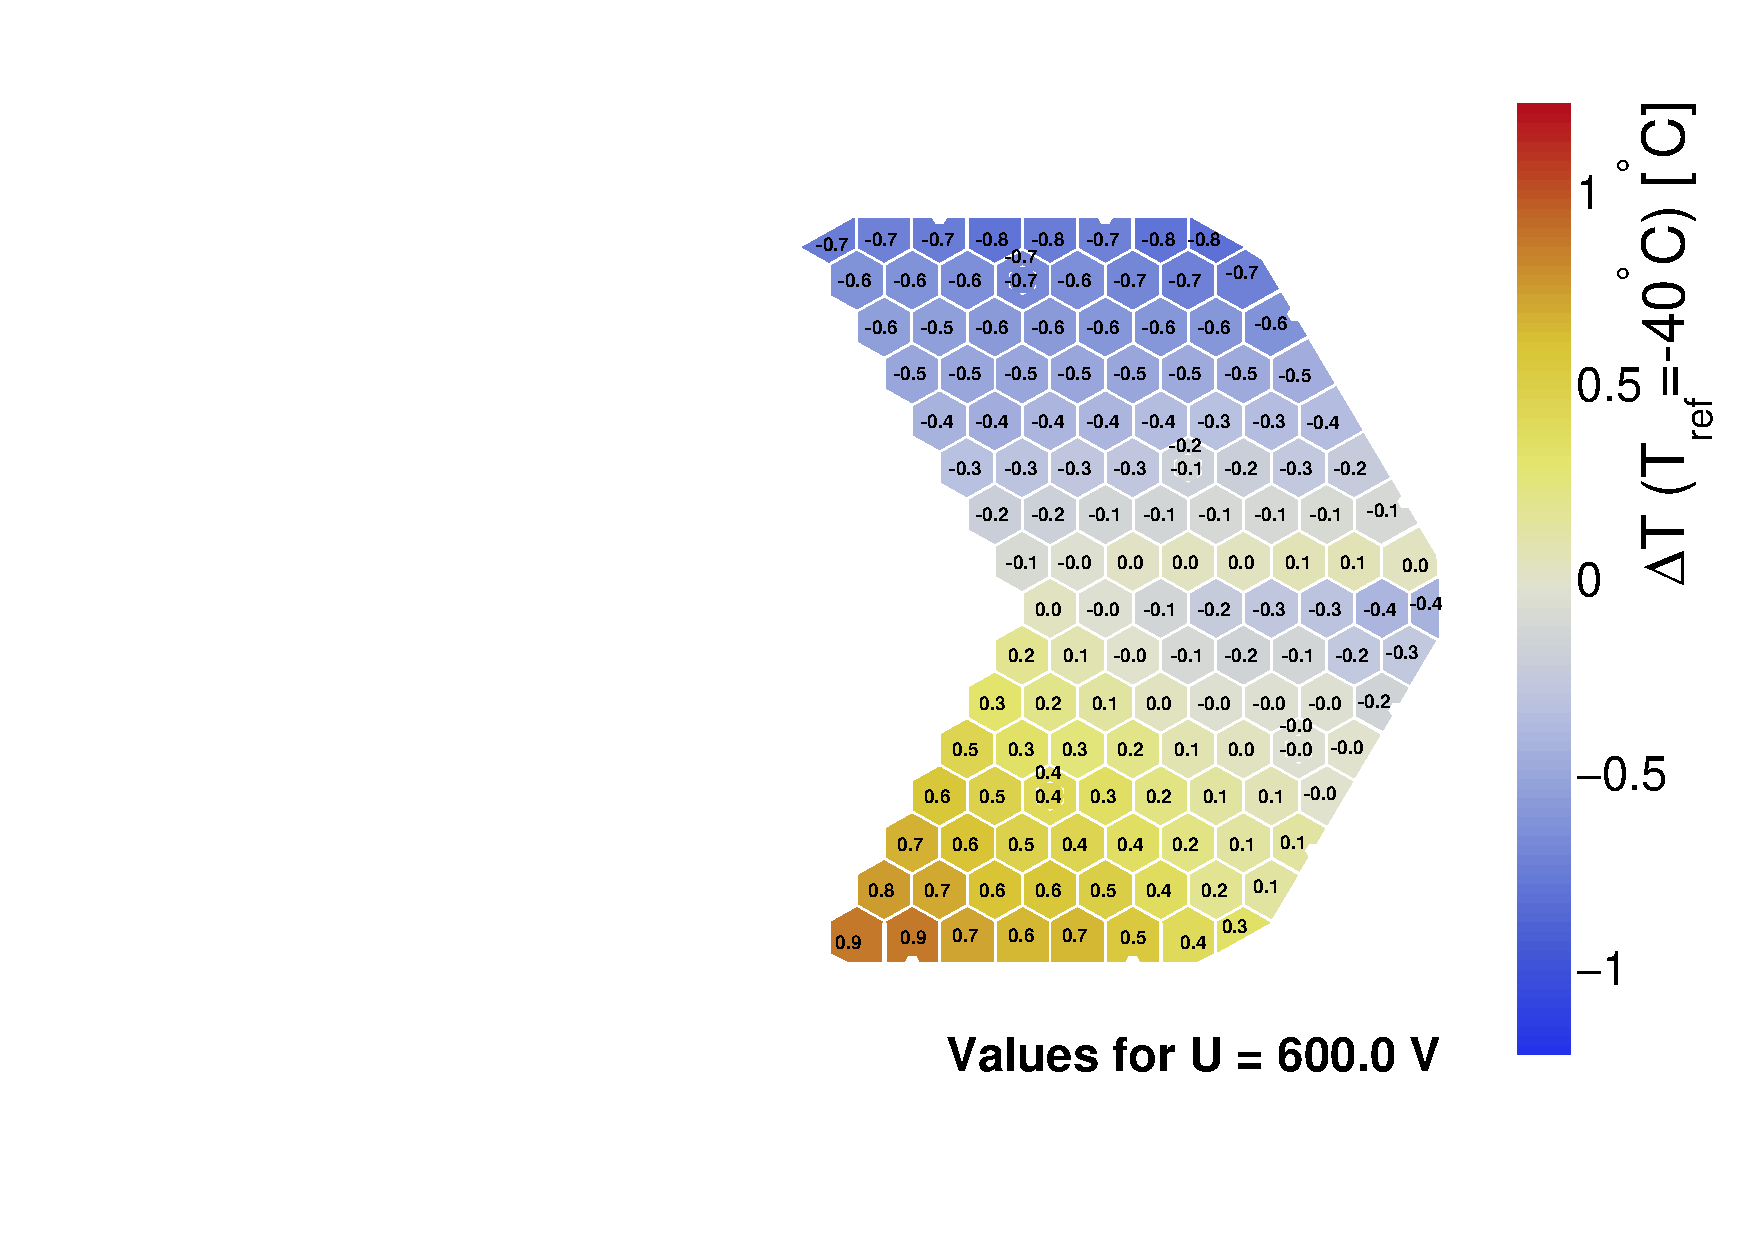
\includegraphics[width=0.999\textwidth]{plots/chuck_temp_correction/Spring2021_ALPS.pdf}
		\subcaption{
		}
		\label{plot:chucktemp_before}
	\end{subfigure}
	\hfill
	\begin{subfigure}[b]{0.32\textwidth}
		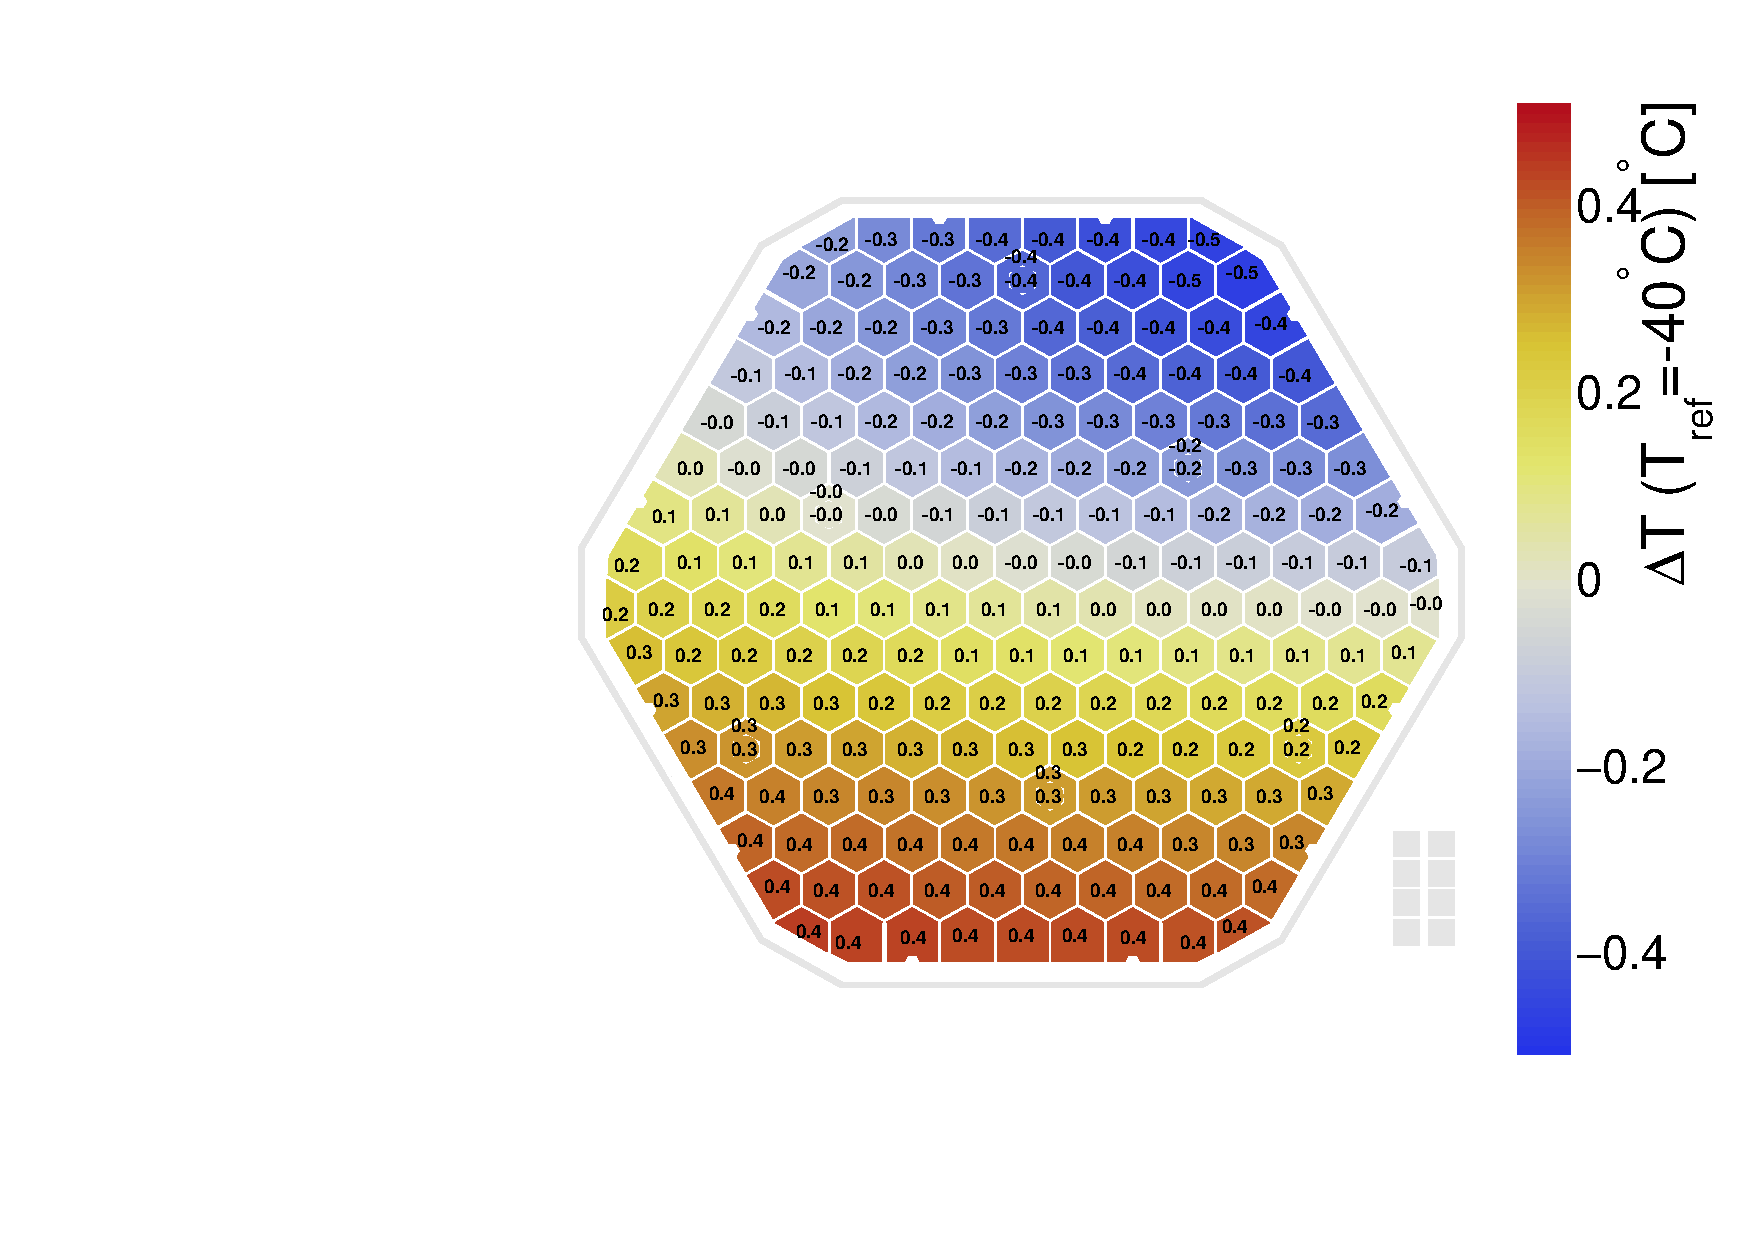
\includegraphics[width=0.999\textwidth]{plots/chuck_temp_correction/Spring2021_ALPS_deltaT.pdf}
		\subcaption{
		}
		\label{plot:chucktemp_correction}
	\end{subfigure}
	\hfill
	\begin{subfigure}[b]{0.32\textwidth}
		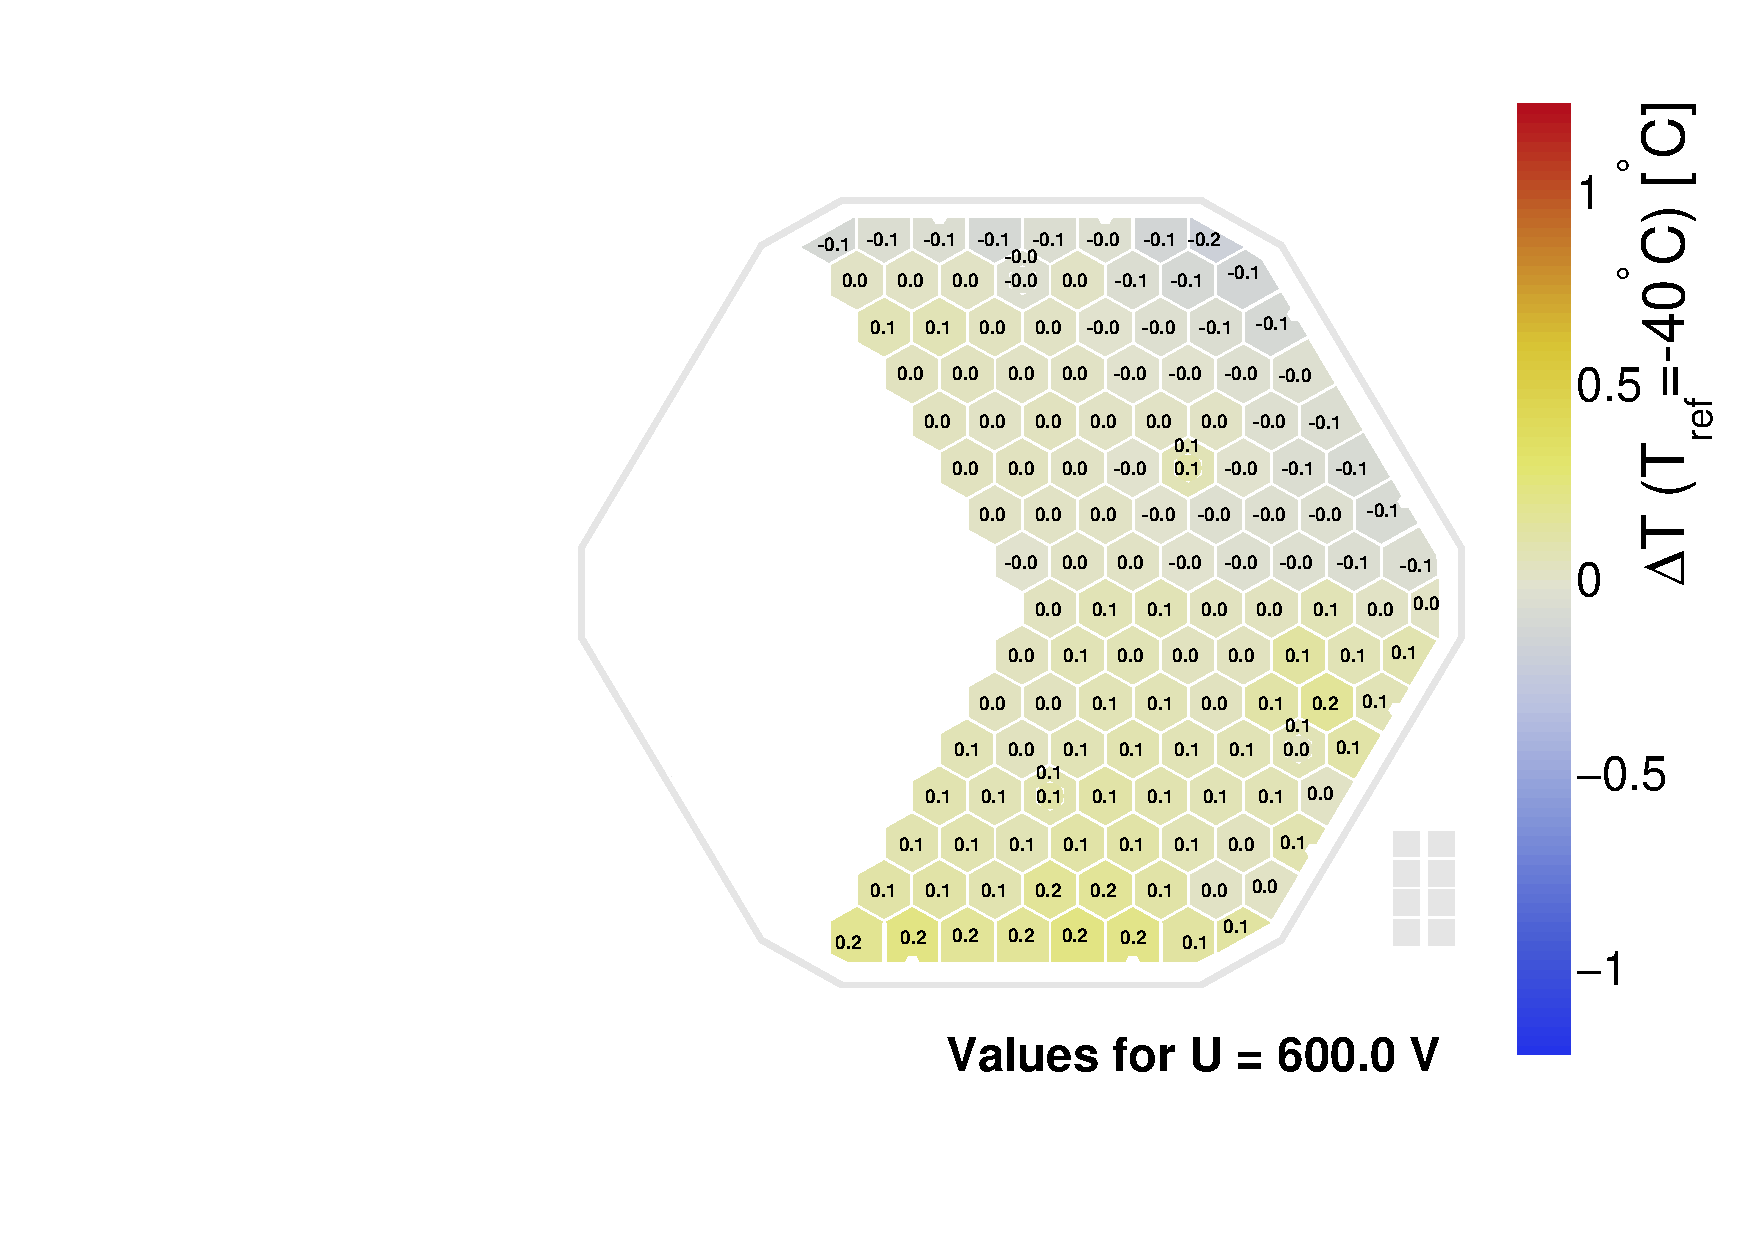
\includegraphics[width=0.999\textwidth]{plots/chuck_temp_correction/Spring2021_ALPS_chucktempcorrected.pdf}
		\subcaption{
		}
		\label{plot:chucktemp_after}
	\end{subfigure}
	\caption{
		Illustration of the chuck temperature inhomogeneity correction (Spring2021-ALPS campaign).
	}
\end{figure}